\section{Peer-to-Peer}

\subsection{Overview P2P systems}
P2P computing is distributed computing  with the following desirable properties:
\begin{itemize}
	\item Resource sharing
	\item Dual client/server role
	\item Decentralization/autonomy
	\item Scalability
	\item Robustness/self-organization
\end{itemize}

\subsection{Distributed Hash Table}

DHT are third generation of P2P:

\begin{tabular}{m{10cm}m{6cm}}
\begin{itemize}
    \item a dynamic distribution of a hash table onto a set of cooperating nodes.
        (different node contains different parts of the table).
    \item Each node has a routing table that points to some other nodes.
    \item Lookup operation is done by node to make a key resolution
\end{itemize}
&
    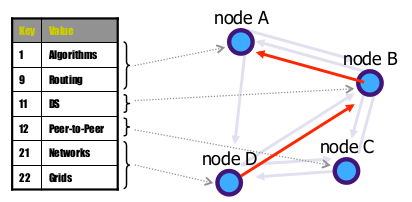
\includegraphics[width=6cm]{img/DHT.png}

     \textcolor{red}{Node D: lookup(9)}\\
    \\
\end{tabular}

\begin{lstlisting}[caption=Interface DHT]
put(key,value).
get(key)
\end{lstlisting}

\subsubsection{Chord}

\begin{tabular}{m{10cm}m{3cm}m{3cm}}
\begin{itemize}
    \item \textbf{Routing table size} $= M$ s.t $N = 2^M$
    \item Every node $n$ know successor $(n + 2^{i-1})$ for $i = 1..M$
    \item $log_2(N)$ maximum hops between two node
\end{itemize}
& 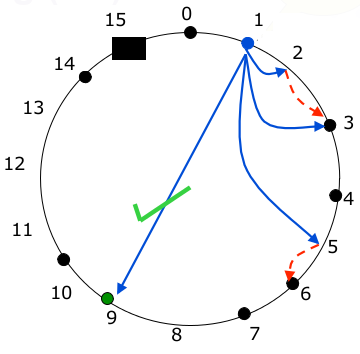
\includegraphics[width=3cm]{img/chord.png}
& 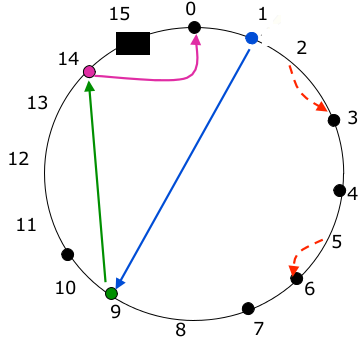
\includegraphics[width=3cm]{img/chord1.png}\\
& \multicolumn{2}{c}{$\Rightarrow$ 1 get(15)}
\end{tabular}

\subsubsection{Generally}

\begin{itemize}
    \item We have $N$ node
    \item[$\to$] Trade-off between lookup length and routing table size

   \begin{eqnarray*}
            H &= log_k(N)\\
            R &=(k-1) H \\
            N &= (\frac{R}{H} + 1)^H\\
        \end{eqnarray*}
\end{itemize}

Chord is a special case where $k=2$.

\subsubsection{DKS}

\begin{itemize}
    \item Tunability: \begin{tabular}{l}
            Routing table size vs lookup length\\
            fault-tolerance degree
        \end{tabular}
    \item Local atomic join and leave (strong guarantees)
    \item Correction-on-use : no unnecessary bandwith consumption
\end{itemize}

\subsubsection{Design DKS(n, k, f)}
\begin{tabular}{m{10cm}m{3cm}m{3cm}}
\begin{itemize}
    \item An \textbf{identifier space} of size $N=k^L$
    \item A hash function
    \item An item ($key, value$) is stored at \textbf{successor} of
        H(key)
    \item \textbf{Bidirectional} linked list of nodes
    \item Resolving key : $\bigoh(N) hops$
\end{itemize}
& 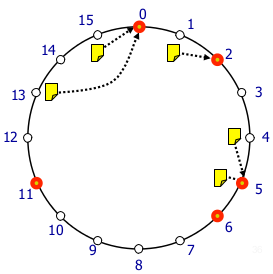
\includegraphics[width=3cm]{img/dks1.png}
& 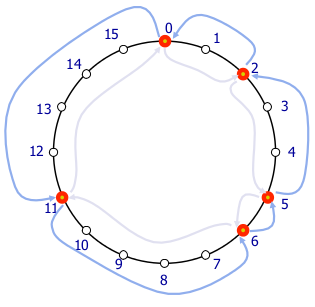
\includegraphics[width=3cm]{img/dks2.png} \\
\end{tabular}


\paragraph{Principle}

\begin{enumerate}
    \item \textbf{Distributed K-ary search}:
        \begin{itemize}
            \item resolution key: $log_k(N)$ hops
            \item At each node, a $RT$ of $\log_k(N)$ level
            \item Each level of $RT$ has $k$ intervals
            \item For level $l$ ant interval $i$: $RT(l)(i) = $ adress of the fist node
                that follow the start of the interval $i$
        \end{itemize}

        \paragraph{Interval routing}
        \begin{enumerate}
            \item If key between my predecessor and me: done
            \item Otherwise systematic forwarding level by level
        \end{enumerate}

        \paragraph{Example with $k=4$, $N=16$}:

        \begin{tabular}{m{6cm}m{6cm}m{4cm}}

            \begin{center}\textcolor{purple}{Level 1} \end{center}
            \begin{eqnarray*}
                I_0 &= [1, 5[ &: RT(1)(0) = 1\\
                I_1 &= [5, 9[ &: RT(1)(1) = 6\\
                I_2 &= [9, 13[ &: RT(1)(2) = 10\\
                I_3 &= [13, 1[ &: RT(1)(3) = 15\\
            \end{eqnarray*}
            &
            \begin{center}\textcolor{green}{Level 2} \end{center}
            \begin{eqnarray*}
                I_0 &= [1, 2[ &: RT(2)(0) = 1\\
                I_1 &= [2, 3[ &: RT(2)(1) = 2\\
                I_2 &= [3, 4[ &: RT(2)(2) = 3\\
                I_3 &= [4, 5[ &: RT(2)(3) = 6\\
            \end{eqnarray*}

            & 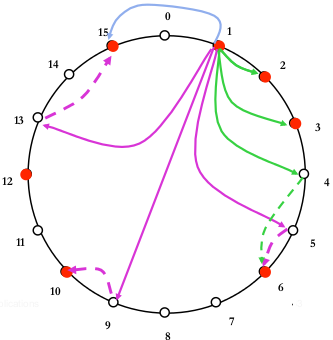
\includegraphics[width=4cm]{img/design1.png}
        \end{tabular}


    \item \textbf{Local atomic action for guarantees}:

        Use local atomic operation for \textbf{join, leave} to ensure
        that any key-value pair previously inserted is found despite concurrent
        joins/leaves.

        \begin{enumerate}
            \item Atomically insterted by it's current successor on the virtual space
            \item New node receive approximate routing information from it's current successor
            \item[$\to$] Concurrent join on the same segment are serialized (because of local
                atomic action)
        \end{enumerate}

        \begin{tabular}{m{10cm}m{4cm}}

            \begin{itemize}
                \item Node 14 join
                \item Pointer for node 1 on level=1 interval=3 become invalid
                \item[$\to$] corrected by correction-on-use
            \end{itemize}

            & 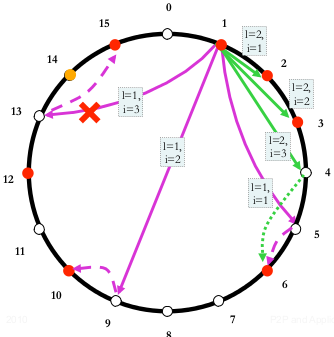
\includegraphics[width=4cm]{img/design2.png}
        \end{tabular}

    \item \textbf{Correction-on-use}:

        \begin{tabular}{m{10cm}m{4cm}}
            Add i (interval) and l (level) with the message
            $\Rightarrow$ $n'$ can comppute $x_i^l(n)$

            \begin{itemize}
                \item[a)] lookup(Key:13, level:1, Interval:3)
                \item[b)] badPointer(Key:13, Candidate:14)
                \item[c)] lookup(Key:13, level:1, Interval:3)
            \end{itemize}

            & 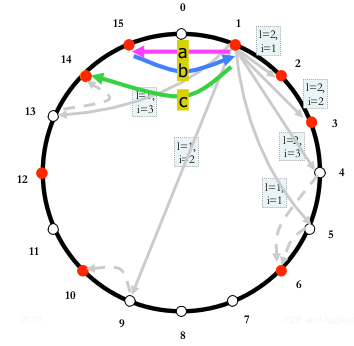
\includegraphics[width=4cm]{img/design3.png}
        \end{tabular}
\end{enumerate}


\subsection{Broadcast in DHTs}

\begin{itemize}
    \item \textbf{DHT as distributed k-ary search}: construct a spanning tree
        derived from the decision tree of the distributed k-ary search after removal
        of the virtual hops

        \paragraph{Invariant}:
        \begin{itemize}
            \item Any node sends to distinct routing entries
            \item Any sender informs receiver about a \textbf{forwarding limit}
            \item[$\to$] Construct disjoint interval and node receives a message once
        \end{itemize}

        \begin{figure}[!ht]
            \centering
            \begin{tabular}{m{4cm}m{4cm}m{4cm}}
                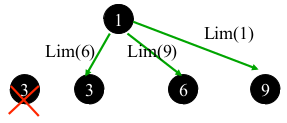
\includegraphics[width=4cm]{img/DHT1.png}
                & 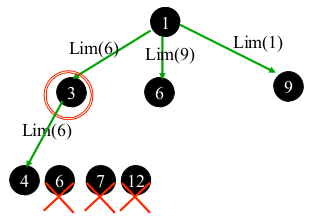
\includegraphics[width=4cm]{img/DHT2.png}
                & 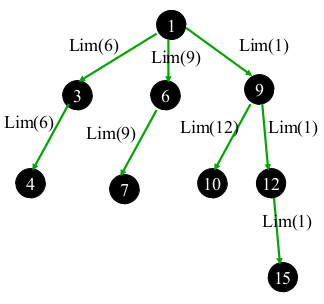
\includegraphics[width=4cm]{img/DHT3.png}\\
            \end{tabular}
            \caption{DHD spanning tree}
        \end{figure}
        \FloatBarrier{}

    \item[Alternative]

    \item \textbf{Gnutella-like flooding in DHT}:
        \begin{itemize}
            \item[Pro] know diameter $\to$ correct TTL $\to$ High guarantees
            \item[Con] High traffic with redundant messages
        \end{itemize}

    \item \textbf{Traversing the ring in Chord or Pastry}:
        \begin{itemize}
            \item[Pro] No redundant message
            \item[Con] Sequential execution time
            \item[Con] Highly sensitive to failure
        \end{itemize}
\end{itemize}


\subsection{Application infrastructure in DHT}
%TODO
